%!TEX root = ../../Master.tex
\section{Organisation}

Det følgende afsnit vil analysere de kontekstuelle forhold for det, som beskrives af Laudon \& Laudon som \enquote{organisation}. Dette vil også inkludere en interessent analyse, i overensstemmelse med rapportens format. Elementer i dette afsnit, beskriver det organisatoriske hierarki i og omkring en havn. Afsnittet er delvist forbundet med menneske afsnittet, og bør læses i forlængelse af hinanden, for at opnå en samlet forståelse.


\subsection{Dansk Sejlunion} % (fold)
\label{sub:Dansk_Sejlunion}

Der eksisterer mange foreninger for både eller sejlskibe i Danmark. En af de største unioner er Dansk Sejlunion (DS), som er et specialforbund under Dansk Idræts Forbund. DS optager klubber i alle former for sejlads som medlemmer. DS har en kollektiv forsikring som alle 273 medlemsklubber automatisk er medlem af, samt andre fordele for medlemsklubberne. Dette inkluderer rabatter på Falcks søsikkerhedspakke, sejlershoppen.dk og Mols-linien, samt juridisk rådgivning \cite{ds_optagelse,ds_fordele}.

Idet DS har så mange medlemsklubber, er denne forening relevant i forhold til at sælge et eventuelt IT-system til sejlklubber i Danmark. DS tilbyder på deres hjemmeside en liste over leverandører af administrationsløsninger til deres medlemmer. Et IT-system på denne liste, vil uden tvivl opnå højere synlighed for eventuelle kunder \cite{DanskSejlunionKlubAdmin}.

% subsubsection Dansk Sejlunion (end)

\subsection{Aalborg/Nørresundby Fritidshavn}

I Aalborg er det kommunen der ejer alle havnene. Aalborg/Nørresundby Fritidshavn (ANF), en paraplyorganisation for bådklubber i Aalborg/Nørresundby, får lov til at bruge disse havne i mod at havnene bliver vedligeholdt. Foreningerne i ANF kan så leje havnene af ANF. Der er typisk én bådklub per havn. Nogle havne benyttes også af mindre klubber som kajakklubber eller søspejdere  \cite{int_vb_sl}.

Der er 4 store lystbådehavne i Aalborg by:
\begin{itemize}[noitemsep]
    \item Marina Fjordpark
    \item Skudehavnen - lystbådehavnsafsnit
    \item Vestre Bådehavn - lystbådehavnsafsnit
    \item Nordre Bådehavn
\end{itemize}



Følgende sejlklubber er medlem af ANF \cite{anf_havnereglement}. Se \cref{fig:anf_overblik}.
\begin{itemize}[noitemsep]
	\item Aalborg Sejlklub
	\item Fiskerklyngen
	\item Vestre Baadelaug
	\item Sejlklubben Limfjorden
	\item Nørresundby Sejlklub
\end{itemize}
 
ANF forestår forhandlinger på vegne af organisationens sejlklubber. En fælles brugsaftale af de fire havne, kan derved indgås med havneejer, Aalborg Kommune.

Indtægterne i ANF består af bådpladsafgifter, som medlemsklubberne skal betale for brug af de tilknyttede havne \cite{anf_budget_2013}. Det er op til de enkle klubber at fordele deres pladser ud til medlemmerne. ANF forpligter sig til vedligeholdelse af havnene tilknyttet foreningen, herunder hovedistandsættelser samt udføring af nyanlæg. \cite{anf_brugsaftale_2012}.

\begin{figure}
  \centering
  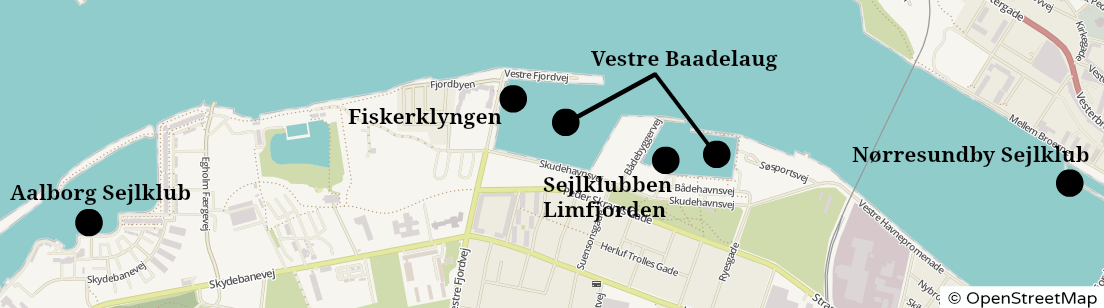
\includegraphics[width=\textwidth]{anf}
 	\caption{Overblik over medlemmerne af ANF} 	\label{fig:anf_overblik}
\end{figure}

% subsection Foreninger (end)


\subsection{Bådklubber}
Her vil vi se på de bådklubber der er tilknyttet Vestre Bådehavn og Skudehavnen, fordi det er disse klubber vi har haft kontakt med.

\subsubsection{Vestre Baadelaug}
Vestre Baadelaug har bådpladser i Vestre Bådehavn og Skudehavnen, som begge deles med Sejlklubben Limfjorden. I Vestre Baadelaug, fordeles disse pladser hvert år ud til medlemmerne. Inden den nye pladsfordeling bliver lavet, er det muligt at ønske en bestemt plads. Der er en masse menneskelige interesser der skal varetages når pladserne skal fordeles. Det er vigtigt for nogle medlemmer hvor de ligger. Det er ikke muligt at få en permanent plads, men kassereren sørger for at et medlem beholder sin tidligere plads når fordelingen bliver lavet. Medlemmerne betaler per\ kvadratmeter. Kvadratmeterne kan opgøres på forskellige måder, for eksempel\ som plads arealet eller som bådarealet. Et medlem kan kun have én bådplads, dog kan der opstå situationer hvor et medlem har mere end en båd, bl.a.\ i forbindelse med salg af en båd. Klubben har omkring 380 medlemmer \cite{int_vb_sl}.

Bestyrelsen i Vestre Baadelaug består af 6 medlemmer, som vælges ind 2 år ad gangen på den ordinære generalforsamling. Bestyrelsen repræsenterer lauget i alle forhold, og beslutninger taget i bestyrelsen forpligter lauget \cite{vestre_vedtagter}.

Som mange andre foreninger, har Vestre Baadelaug en formand og en næstformand. Formandens opgave er at repræsentere foreningen udadtil, herunder også i retsforhold. Derudover koordinerer formanden bestyrelsens arbejde. Formanden har den afgørende stemme i tilfælde af stemmelighed i bestyrelsen. Næstformanden er suppleant til formanden, og kan træde i formandens sted. Derudover hjælper næstformanden generelt til i foreningen \cite{vestre_vedtagter}.

Sekretæren i Vestre Baadelaug sørger for at tage referat af alle møder i bestyrelsen og generalforsamlingen, og sørger for at distribuere disse referater. Udover dette, fungerer sekretæren også som ansvarshavende redaktør på klubblad \cite{vestre_vedtagter}.

Klubbens regnskabs og medlemsprotokol udføres af kassereren. Når et nyt medlem skal indmeldes, er dette kassererens ansvarsområde. Dertil skal kassereren administrere og betale regninger for klubben \cite{int_vb_sl}.

\subsubsection{Sejlkubben Limfjorden}
Sejlkubben Limfjorden har omkring 150 medlemmer \cite{int_vb_sl}. Klubbens medlemmer omfatter kun personer med sejlbåde. Klubben er medlem af Dansk Sejlunion. Sejlklubben deler Vestre Bådehavn, Skudehavnen og havnefoged med Vestre Baadelaug, hvilket betyder at nogle administrationsopgaver deles af begge klubber. 

%% Fr: det skal vi nok ikke havde med
%\subsubsection{Aalborg Sejlklub}
%Aalborg Sejlkulb er en Sejlklub, der hører til i havnen Marina Fjordparken. Nørresundby Sejlklub er tilknyttet Nørresundby havn. Klubben er medlem af Danske Tursejlere \cite{norresundby_sejlklub}.

\subsection{Regler og love}
Transportministeriet har i 2002 udgivet en bekendtgørelse om standardreglement for lystbådehavne \cite{standardreglement}. I denne er der regler om hvordan medlemmer, samt gæster skal opføre sig når de befinder sig i en havn. De enkelte havne skal udarbejde et individuelt ordensreglement, som beskriver hvilket område det gælder for, og hvilke særlige ordensregler der skal gælde på havnen. Derudover skal det referere til bekendtgørelsen.

I standardreglementet bliver der beskrevet hvordan fartøjet skal fortøjes og hvordan der skal sejles i havne. Blandt andet står der at gæstende fartøjer skal melde deres ankomst til havnemyndigheden, og de skal flytte deres fartøj til en anden plads hvis havnemyndigheden siger det. Føreren af ethvert fartøj har også pligt til jævnligt at holde øje med sit fartøj, når det ligger i havnen. Fartøjet skal være forsvarligt fortøjret og tove skal fastgøres så de ikke klapper mod masten. I reglementet er der regler for optagning, reparation, brændstof og forskellige miljøbestemmelser.

Ifølge standardreglementet er det havnemyndigheden der står for at holde orden på et havneområdet. Enhver som befinder sig på havneområdet skal overholde havnemyndighedens anvisninger. Politiet og andre myndigheder skal stadigvæk udføre deres opgaver inden for deres lovgivningsmæssige regler. De fleste regler i standardreglementer kan omgås hvis der gives tilladelse fra havnemyndigheden. Hvis en regel ikke bliver overholdt kan havnemyndigheden flytte den pågældende båd for ejerens regning.


\subsection{Aalborg Kommune}

Aalborg Kommune er kendt i Danmark som en uddannelsesby på grund af Aalborg Universitet. Aalborg Kommune ligger stor vægt på at byen skal være attraktiv for studerende, ved at prioritere ungdomsboliger og universitets velvære højt \cite{udd-strat-aalborg}. Aalborg Kommune forsøger at få et mere \enquote{alsidigt og nyskabende kulturliv} \cite{aalborgKulturPolitik}, og de har sat 310 millioner kroner af til at forbedre Aalborgs kulturliv. Heriblandt indgår Aalborgs rige havnemiljø, med bådklubber, besøgende krydstogter og havnefronten \cite{AalborgHavnefront}. For at opnå et levende og kreativt kulturmiljø er Aalborg Kommune interesseret i bådklubbernes velvære og funktionalitet.

